%-------------------------------------------------------------------------------
%                            BAB III
%               		METODOLOGI PENELITIAN
%-------------------------------------------------------------------------------
\fancyhf{}
\fancyfoot[C]{\thepage}
\chapter{METODOLOGI PENELITIAN}

\section{\uppercase{WAKTU DAN LOKASI PENELITIAN}}
\setlength\parindent{30pt} Penelitian ini dilaksanakan di lantai 1 dan 3 di Gedung A FMIPA Universitas Syiah Kuala (USK). Waktu yang dibutuhkan untuk penelitian ini terhitung dari bulan Oktober 2021 hingga Mei 2022.

% \par Rincian penelitian dapat dilihat pada tabel \ref{tabelwaktupenelitian}
% \begin{table}[H]
% 	\centering 
% 	\small
% 	\fontsize{10pt}{20pt}
% 	\selectfont
% 	\caption{Jadwal Penelitian}
% 	\begin{tabular}{|c|l|rlllll|lllll|}
% 	\hline
% 						  & \multicolumn{1}{c|}{}                             & \multicolumn{6}{c|}{Bulan/Tahun 2021}                                                                                                                                                                                                                                                           & \multicolumn{5}{c|}{Bulan/Tahun 2022}                                                                                                                                                                                    \\ \cline{3-13} 
% 	\multirow{-2}{*}{No.} & \multicolumn{1}{c|}{\multirow{-2}{*}{Keterangan}} & \multicolumn{1}{c|}{7}                                               & \multicolumn{1}{c|}{8}                        & \multicolumn{1}{c|}{9}                        & \multicolumn{1}{c|}{10}                       & \multicolumn{1}{c|}{11}                       & \multicolumn{1}{c|}{12}  & \multicolumn{1}{c|}{1}                        & \multicolumn{1}{c|}{2}                        & \multicolumn{1}{c|}{3}                        & \multicolumn{1}{c|}{4}                        & \multicolumn{1}{c|}{5}   \\ \hline
% 	1                     & Studi Literatur                                   & \multicolumn{1}{r|}{\cellcolor[HTML]{656565}{\color[HTML]{9B9B9B} }} & \multicolumn{1}{l|}{\cellcolor[HTML]{656565}} & \multicolumn{1}{l|}{}                         & \multicolumn{1}{l|}{}                         & \multicolumn{1}{l|}{}                         &                          & \multicolumn{1}{l|}{}                         & \multicolumn{1}{l|}{}                         & \multicolumn{1}{l|}{}                         & \multicolumn{1}{l|}{}                         &                          \\ \hline
% 	2                     & Penulisan Proposal                                & \multicolumn{1}{r|}{}                                                & \multicolumn{1}{l|}{\cellcolor[HTML]{656565}} & \multicolumn{1}{l|}{\cellcolor[HTML]{656565}} & \multicolumn{1}{l|}{}                         & \multicolumn{1}{l|}{}                         &                          & \multicolumn{1}{l|}{}                         & \multicolumn{1}{l|}{}                         & \multicolumn{1}{l|}{}                         & \multicolumn{1}{l|}{}                         &                          \\ \hline
% 	3                     & Pengembangan Aplikasi                             & \multicolumn{1}{r|}{}                                                & \multicolumn{1}{l|}{}                         & \multicolumn{1}{l|}{\cellcolor[HTML]{656565}} & \multicolumn{1}{l|}{\cellcolor[HTML]{656565}} & \multicolumn{1}{l|}{\cellcolor[HTML]{656565}} &                          & \multicolumn{1}{l|}{}                         & \multicolumn{1}{l|}{}                         & \multicolumn{1}{l|}{}                         & \multicolumn{1}{l|}{}                         &                          \\ \hline
% 	4                     & Evaluasi Sistem                                   & \multicolumn{1}{r|}{}                                                & \multicolumn{1}{l|}{}                         & \multicolumn{1}{l|}{}                         & \multicolumn{1}{l|}{}                         & \multicolumn{1}{l|}{\cellcolor[HTML]{656565}} & \cellcolor[HTML]{656565} & \multicolumn{1}{l|}{\cellcolor[HTML]{656565}} & \multicolumn{1}{l|}{}                         & \multicolumn{1}{l|}{}                         & \multicolumn{1}{l|}{}                         &                          \\ \hline
% 	5                     & Penulisa Laporan Akhir                            & \multicolumn{1}{l|}{}                                                & \multicolumn{1}{l|}{}                         & \multicolumn{1}{l|}{}                         & \multicolumn{1}{l|}{}                         & \multicolumn{1}{l|}{}                         & \cellcolor[HTML]{656565} & \multicolumn{1}{l|}{\cellcolor[HTML]{656565}} & \multicolumn{1}{l|}{\cellcolor[HTML]{656565}} & \multicolumn{1}{l|}{\cellcolor[HTML]{656565}} & \multicolumn{1}{l|}{\cellcolor[HTML]{656565}} & \cellcolor[HTML]{656565} \\ \hline
% 	\end{tabular}
% 	\end{table}

\section{\uppercase{ALAT DAN BAHAN}}
Alat dan bahan yang digunakan pada penelitian ini meliputi perangkat keras, perangkat lunak dan bahan yang mendukung pada penelitian ini adalah data \textit{Received Signal Strength Indicator} (RSSI) dari hasil survei di lokasi penelitian. Adapun perangkat lunak yang digunakan adalah:
\begin{itemize}
	\itemsep0em
	\item OS Windows 10.
	\item Google Chrome.
	\item Visual Studio Code 1.59.1
	\item React Native
	\item MongoDB Compass 1.28.1
	\item Figma
	\item Postman 8.12.0
\end{itemize}

\par Sedangkan komponen perangkat keras yang digunakan meliputi 1 unit Laptop Acer dengan RAM 3GB, Intel® Core™ i3-3230M CPU @2.60Ghz (4 CPUs), ~2.6 GHz Processor, \textit{Harddisk} 500GB, \textit{Solid State Drive} (SSD) 120GB, memiliki Sistem Operasi Windows 64-bit, 31 unit \textit{Beacon}, serta smartphone Samsung A30.

\section{\uppercase{METODE PENELITIAN}}
Metode penelitian yang dilakukan terdiri dari beberapa tahapan. Skema dari alur tahapan tersebut dapat dilihat pada Gambar \ref{metpen}.
\begin{figure}[H]
	\centering
	{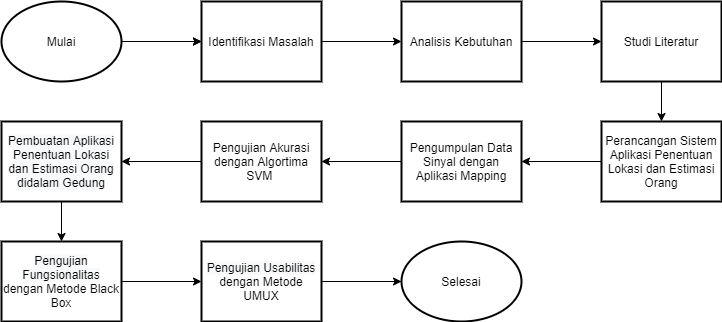
\includegraphics [width = 14cm, height= 6cm]{gambar/metodepenelitian.drawio }}
	\caption{Diagram Alir Penelitian}
	\label{metpen}
\end{figure}

\fancyhf{}
\fancyfoot[R]{\thepage}

\subsection{Identifikasi Masalah}
Tahapan ini adalah proses mengidentifikasi masalah sehingga aplikasi ini perlu dibuat. Adapun masalah yang diidentifikasikan adalah sebagai berikut:
\begin{enumerate}[1.]
	\itemsep0em
	\item Global Positioning System (GPS) belum bisa berfungsi jika digunakan dalam gedung.
	      \citep{Keluza2017}.
	\item Perlunya data estimasi orang dalam gedung untuk pencegahan Covid-19
	\item Belum tersedia Aplikasi Penentuan Lokasi dan Estimasi Orang dalam Gedung .
\end{enumerate}

%%%%%%%%%%%%%%%%%%%%%%%%%%%%%%%%%%%%%%%%%%%
\subsection{Analisis Kebutuhan}
Pada tahapan ini, analisa kebutuhan bersumber dari masalah yang telah diidentifikasi pada tahap sebelumnya sehingga perancangan aplikasi dibangun sesuai kebutuhan. Adapun kebutuhan dari sistem yang dibangun adalah sebagai berikut:

\par \textbf{Kebutuhan Fungsional} Kebutuhan fungsional adalah fungsionalitas sistem itu sendiri. Adapun kebutuhan fungsional dari identifikasi masalah yang telah dilakukan adalah sebagai berikut:

\begin{itemize}
	\item Melakukan proses penentuan lokasi pengguna di dalam gedung FMIPA USK berbasis Crowdsourcing Indoor Localization System.

	\item Menampilkan data estimasi orang di dalam gedung FMIPA USK.

\end{itemize}

\par \textbf{Kebutuhan Non-Fungsional} Kebutuhan non-fungsional memastikan batasan eksternal yang harus dipenuhi oleh sistem. Batasan-batasan tersebut antara lain:
\begin{itemize}
	\item System hanya dapat mendeteksi lokasi pengguna di dalam gedung yang telah dipetakan

	\item Dapat melakukan proses penentuan lokasi apabila bluetooth pada perangkat hidup dan terkoneksi dengan internet.

	\item Dapat mendata estimasi orang di dalam gedung.

\end{itemize}



%%%%%%%%%%%%%%%%%%%%%%%%%%%%%%%%%%%%%%%%%
\subsection{Studi Literatur}
Pada proses studi literatur, peneliti mengumpulkan bahan referensi penelitian yang bersumber dari jurnal-jurnal nasional dan internasional yang terkait penelitian ini dan situs \textit{website} serta buku-buku referensi untuk penelitian ini. Studi literatur dikembangkan untuk menyempurnakan penelitian sebelumnya.

\subsection{Perancangan Sistem Aplikasi Penentuan Lokasi dan Estimasi Orang}
Pada tahap ini, peneliti merancang alur kerja  sistem sehingga bisa memastikan sistem yang dirancang dapat digunakan sesuai kebutuhan pengguna. Alur kerja sistem dijelaskan menggunakan diagram alir yang dapat dilihat dari gambar berikut ini.
\ref{alur-kerja-sistem}.

\begin{figure}[H]
	\centering
	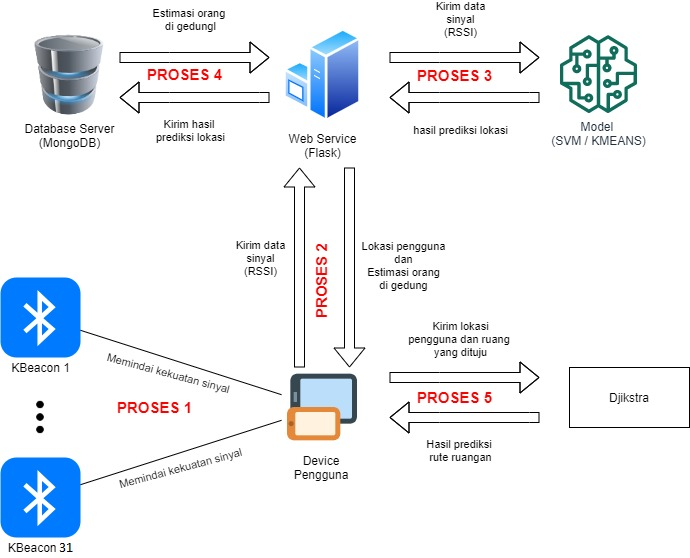
\includegraphics[width=10cm, height=8cm]{gambar/alurkerja.jpeg}
	\caption{Alur Kerja Sistem.}
	\label{alur-kerja-sistem}
\end{figure}

\subsection{Pengumpulan Data Sinyal dengan Aplikasi \textit{Mapping}}
\par Untuk memperoleh dataset untuk penelitian ini, maka diperlukan aplikasi \textit{mapping} untuk menangkap sinyal \text{bluetooth} dari alat \textit{Beacon}. Aplikasi \textit{mapping} ini juga sudah memiliki sertifikat Hak Kekayaan Intelektual (HKI) dengan nomor EC00201972853. Nilai RSSI yang diperoleh dari 31 \textit{Beacon} yang dipasang dari setiap sudut ruangan akan disimpan dalam database mongoDB.
\par Pada penelitian sebelumnya, aplikasi \textit{mapping} menyimpan data di local server sehingga  tidak efektif jika digunakan oleh banyak server. Oleh karena itu, penulis merancang \textit{Web Service} agar data yang disimpan saat penelitian atau \textit{mapping} akan disimpan di database \textit{mongoDB}. Adapun fitur yang tersedia pada aplikasi \textit{mapping} ini adalah:

\begin {itemize}
\itemsep0em
\item Pemindaian Kekuatan Sinyal \newline
Aplikasi ini akan melakukan pemindaian kekuatan sinyal yang ditangkap dari setiap \textit{beacon} yang ditempel di setiap sudut ruangan, sehingga bisa menampilkan data RSSI, label, \textit{Mac Address}, nama \textit{beacon} yang ditandai tersebut.

\item Menyimpan Data Kekuatan Sinyal \newline
Ketika selesai melakukan \textit{mapping}, data kekuatan sinyal disimpan ke database \textit{mongoDB} yang berada di server. Data tersebut akan digunakan pada tahap penelitian selanjutnya.
\end{itemize}


\par Adapun proses pengumpulan data sinyal secara detail, dijelaskan tahapannya sebagai berikut:
\begin{enumerate}[a.]
	\itemsep0em
	\item Pengukuran Jarak Lokasi Penelitian
	      \\
	      Pengukuran ini bertujuan untuk mengukur jarak dari denah lokasi penelitian yang telah dibuat. Hal ini agar bertujuan untuk membuat bobot pada algoritma \textit{Support Vector Machine} (SVM).
	\item Pembuatan Denah Lokasi Penelitian
	      \\
	      Pembuatan Denah Lokasi Penelitian didasarkan pada rancangan gedung FMIPA USK. Denah ini bertujuan untuk menentukan posisi \textit{reference point} untuk proses pemetaan nantinya.
	\item Penentuan Letak \textit{Reference Point}
	      \\
	      Pada tahap ini, letak \textit{reference point} berada di gedung Blok A FMIPA USK, di antaranya adalah di lantai 1, tangga lantai 1 menuju lantai 2, tangga lantai 2 menuju lantai 3, koridor depan Laboratorium Jaringan Komputer, Laboratorium Database, dan Laboratorium Sistem Informasi Geografis.Penentuan letak \textit{reference point} ini dilakukan di setiap sudut ruangan kecuali di dalam ruangan laboratorium. Penentuan \textit{reference point} dilakukan secara urut dengan masing-masing jarak antara satu \textit{reference point} ke \textit{reference point} yang lain sejauh 2 ubin lantai atau 120 centimeter untuk meminimalisir \textit{position error}. \citep{Lee2019} \citep{Bahl2000}. Tujuan penentuan posisi \textit{reference point} ini bertujuan untuk menentukan lokasi pengumpulan data kekuatan sinyal yang dipancarkan setiap \textit{Beacon} di setiap sudut ruangan. Penentuan \textit{reference point} yang saling berdekatan mempengaruhi hasil tahap \textit{positioning}. Denah lokasi penelitian ini dapat dilihat pada Gambar \ref{gedungA}.

	      %\vspace{2cm}
	      \begin{figure}[H]
		      \centering
		      \subfloat[Denah Lantai 1]{{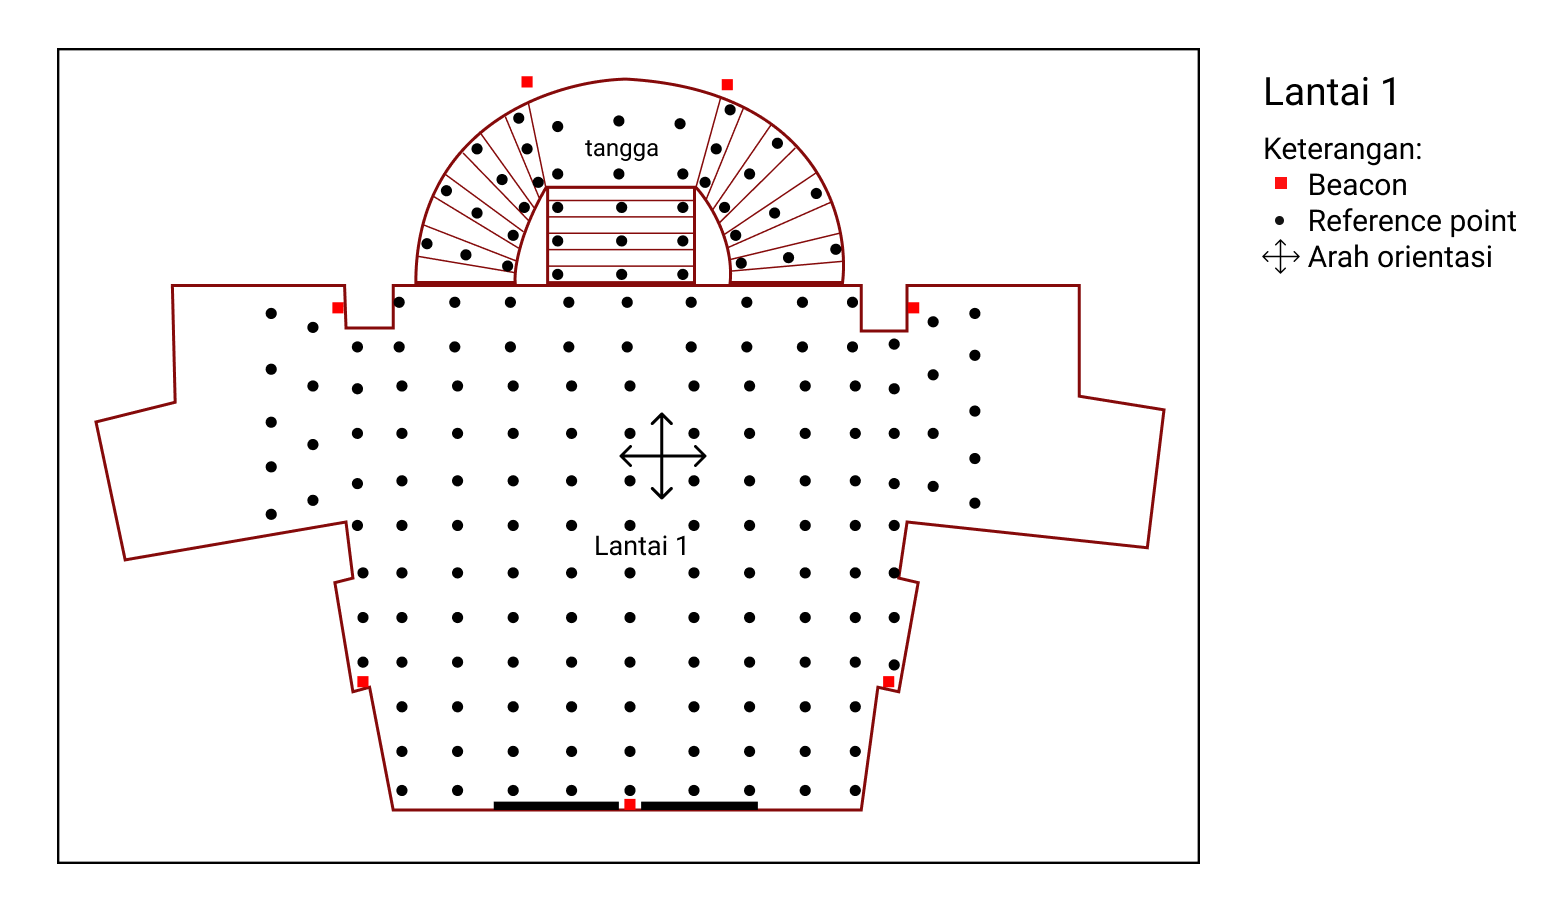
\includegraphics[width=13cm, height=7cm]{gambar/Lantai1} }}%
		      \qquad
		      \subfloat[Denah Lantai 2]{{\includegraphics[width=13cm, height=8cm]{gambar/lantai2} }}

		      \centering
		      \subfloat[Denah Lantai 3]{{\includegraphics[width=12cm, height=6cm]{gambar/lantai3} }}
		      \caption{Ilustrasi Denah Lokasi Letak \textit{Reference Point} Penelitian Gedung Blok A FMIPA USK}%
		      \label{gedungA}%
	      \end{figure}

	      \par Pada proses ini, masing-masing \textit{reference point} saat mengambil kekuatan sinyal akan menghadap 4 arah oriental yaitu depan, belakang, kiri dan kanan. Tiap arah orientasi, antena \textit{host} yang dimiliki oleh \textit{smartphone} memiliki konektivitas \textit{line-of-sight} (LoS) ke sebuah antena \textit{Beacon} selama orientasinya berlawanan. Arah orientasi dari tubuh pengguna juga dapat menimbulkan halangan dan kekuatan sinyal yang ditangkap juga berbeda. Oleh karena itu, perlu dilakukan pencatatan \textit{direction} (d), dengan menghadap ke depan, ke kanan, ke belakang dan ke kiri tergantung pada pengambilan kekuatan sinyal yang dilakukan \citep{christ1993}. Metode pengambilan kekuatan sinyal setiap \textit{Beacon} berdasarkan proses survei pemetaan \textit{reference point} disebut dengan metode \textit{Fingerprinting}. Metode \textit{Fingerprinting} dilakukan dengan mengumpulkan  data-data kekuatan sinyal tersebut ke dalam basis data \textit{mongoDB} untuk dijadikan sebagai data \textit{training} nantinya.

	      %%%%%%%%%%%%%%%%%%%%%%next%%%%%%%%%%%%%%%%%%%%%
	\item Pengumpulan Data \textit{Training}
	      \par
	      Basis data yang berisikan data \textit {training} yaitu data kekuatan sinyal dengan nilai RSSI yang didapatkan dari tiap \textit{beacon} dilakukan berdasarkan penentuan letak \textit{reference point} yang telah ditentukan pada tahap sebelumnya. Pengumpulan data \textit{training} dengan pemetaan metode \textit{Fingerprinting} ini menggunakan Aplikasi \textit{Mapping} yang telah dibuat dengan fitur-fitur untuk dapat menangkap kekuatan sinyal dari \textit{Beacon}, kemudian informasi-informasi dari \textit{Beacon} tersebut seperti MAC Address, nilai RSSI, dan nama ruangan dimana kekuatan sinyal tersebut ditangkap dapat disimpan pada server. Ilustrasi penyimpanan data \textit{training} dengan metode \textit{Fingerprinting} untuk \textit{reference point} dapat dilihat pada Tabel \ref{fingerprinting}. Orientasi yang tercantum pada gambar tersebut hanya sebagai gambaran bahwa penyimpanan data terhadap suatu posisi diambil berdasarkan 4 arah orientasi.

	      \begin{landscape}
		      \begin{table}[H]
			      \caption{Ilustrasi Penyimpanan Data Training Metode \textit{Fingerprinting} pada \textit{Reference Point}}
			      \centering
			      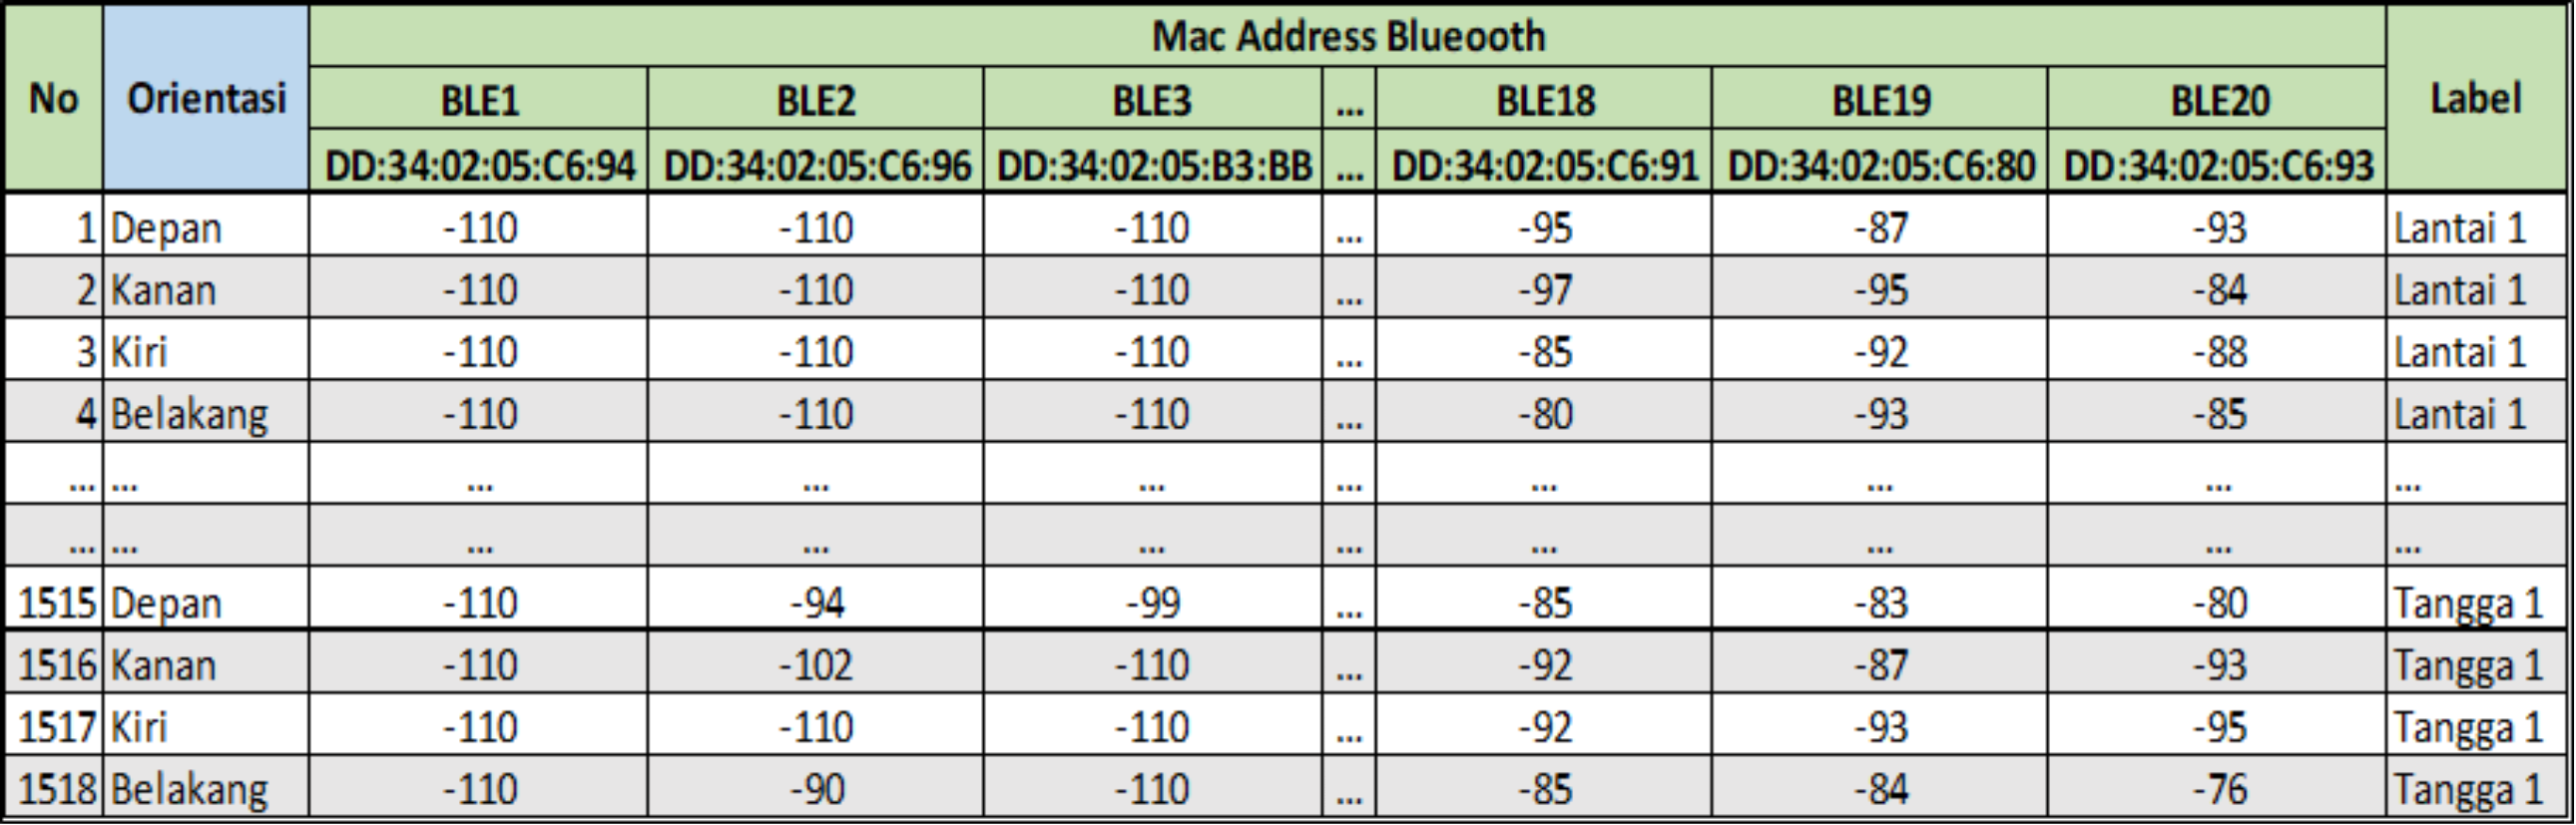
\includegraphics[width=25cm, height=7cm]{gambar/tes}
			      \label{fingerprinting}
		      \end{table}
	      \end{landscape}



	      \vspace{3cm}

	\item Pengumpulan Data Uji
	      \\
	      Pengumpulan data uji dilakukan setelah pengumpulan data \textit{training}. Data uji bertindak seolah-olah kelas label belum diketahui. Data uji tersebut akan dibandingkan dengan data \textit{training}, hasil tersebut akan diimplementasikan pada Aplikasi Penentuan Lokasi dan Estimasi Orang di dalam Gedung untuk memprediksi lokasi pengguna dengan metode klasifikasi \textit{Support Vector Machine} (SVM).

\end{enumerate}
%%%%%%%%%%%%%%%%%%%%%%%%%%%%%%%%%%%%%%%%%%%%%%%%%%%%%%%%%%%%%%%%%%%%%%%%%%%%%%%%%%%%%%%%%%%%%%%%%%%%%%%%%%%%%%%%%%%%%%%%%%%
%TESTING svm%
\subsection{Pengujian Akurasi dengan Algoritma SVM}

\par Pengujian ini dilakukan dengan tujuan untuk mengetahui tingkat keberhasilan prediksi dengan menggunakan algoritma \textit{Support Vector Machine} (SVM) terhadap lokasi pengguna berdasarkan \textit{reference point} yang digunakan. Algoritma klasifikasi SVM pada penelitian ini dibuat dengan menggunakan kode Python. Algoritma SVM pada penelitian ini bersifat sekali training dikarenakan menggunakan \textit{library} Python scikit learn dan menghasilkan pickle bukan model. Pickle tidak bersifat real time dan jika ingin memperbarui file harus melakukan proses \textit{training} ulang. Adapun denah untuk kelas pada algoritma SVM dapat digambarkan pada gambar \ref{gedungA}.

\par Peran algoritma SVM pada penelitian ini sangat penting, diantaranya yang pertama adalah pada saat proses klasifikasi. Klasifikasi menggunakan algoritma SVM sangat penting pada proses \textit{training} dan \textit{testing} sehingga menghasilkan nilai akurasi dan \textit{pickle}. Kemudian peran SVM ini juga digunakan pada proses prediksi lokasi pengguna yang sedang berada di dalam gedung dan juga memiliki peran dalam menentukan estimasi jumlah orang di dalam gedung, dimana pickle SVM di simpan pada \textit{web service}.

\par Proses prediksi menggunakan algoritma SVM ini adalah pertama sinyal yang ditransmisikan tiap beacon akan ditangkap oleh perangkat Android si pengguna lalu data sinyal RSSI tersebut dikirim ke \textit{web service flask} agar di klasifikasi dan diprediksi oleh algoritma SVM. Kemudian hasil prediksi tersebut dikirim ke database server, jika hasil prediksi tersebut adalah di dalam gedung FMIPA maka akan masuk ke dalam estimasi jumlah orang di dalam gedung dan sebaliknya jika hasil prediksinya adalah di luar FMIPA maka tidak dimasukkan ke dalam estimasi jumlah orang di dalam gedung. Sehingga hasil prediksi lokasi pengguna dan estimasi jumlah orang di dalam gedung akan di tampilkan di output aplikasi.


%\vspace{2cm}
% \begin{figure}[H]
% 	\centering
% 	\subfloat[Denah kelas SVM Lantai 1]{{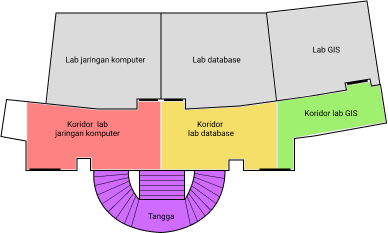
\includegraphics[width=16cm, height=8cm]{gambar/class1.png} }}%
% 	\qquad
% 	\subfloat[Denah kelas SVM Lantai 2]{{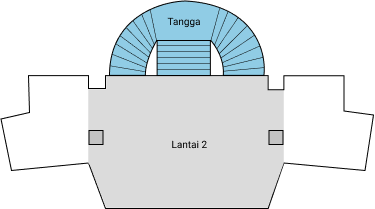
\includegraphics[width=18cm, height=9cm]{gambar/class2.png} }}
% 	\centering
% 	\subfloat[Denah kelas SVM Lantai 3]{{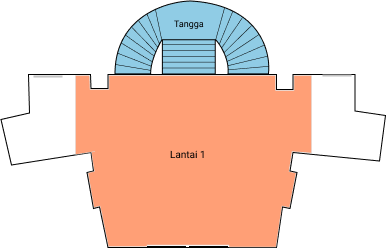
\includegraphics[width=18cm, height=9cm]{gambar/class3.png} }}
% 	\caption{Ilustrasi Denah Menggambarkan Kelas SVM}%
% 	\label{gedungA}%
% \end{figure}

\begin{figure}[H]
	\centering
	\subfloat[Denah Lantai 1]{{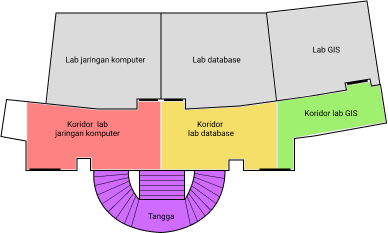
\includegraphics[width=13cm, height=7cm]{gambar/class1.png} }}%
	\qquad
	\subfloat[Denah Lantai 2]{{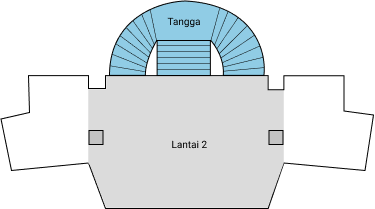
\includegraphics[width=13cm, height=8cm]{gambar/class2.png} }}

	\centering
	\subfloat[Denah Lantai 3]{{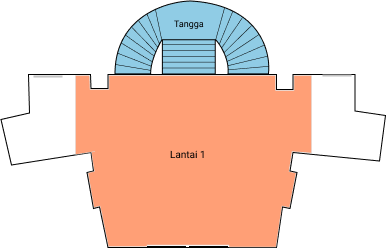
\includegraphics[width=12cm, height=6cm]{gambar/class3.png} }}
	\caption{Ilustrasi Denah Menggambarkan Label SVM}%
	\label{gedungA}%
\end{figure}


\subsection{Pembuatan Aplikasi Penentuan Lokasi dan Estimasi Orang di dalam Gedung}
\par Aplikasi Penentuan Lokasi dan Estimasi Jumlah Orang di dalam Gedung dibangun menggunakan \textit{react native} ini adalah aplikasi berbasis Android yang berguna untuk mempermudah pengguna dan rekan tim penelitian untuk melakukan proses pencarian lokasi dan estimasi jumlah orang yang berada di dalam gedung Blok A Fakultas Matematika dan Ilmu Pengetahuan Alam Universitas Syiah Kuala, yang dikembangkan dengan konsep \textit{Indoor Localization System} dan \textit{Crowdsourcing}. Aplikasi ini bekerja apabila perangkat smartphone sudah mendukung Bluetooth 4.0, dikarenakan aplikasi ini menangkap kekuatan sinyal atau nilai RSSI dari \textit{Beacon} yang terintegrasi BLE di dalamnya. Kekuatan sinyal yang ditangkap akan dilakukan perhitungan menggunakan metode klasifikasi \textit{Support Vector Machine} (SVM), output dari perhitungan tersebut adalah prediksi lokasi pengguna yang akan dikirim ke \textit{web services flask} secara background process. Adapun fitur-fitur yang tersedia adalah sebagai berikut:

\begin {itemize}
\itemsep0em
\item Memprediksi Lokasi Pengguna saat berada di dalam gedung
\item Menampilkan Estimasi Jumlah Orang yang Berada di dalam Gedung Blok A Fakultas Matematika dan Ilmu Pengetahuan Alam Universitas Syiah Kuala
\end{itemize}

\par Proses penentuan lokasi pada penelitian ini adalah bagaimana sistem melacak keberadaan pengguna yang menggunakan aplikasi ini saat berada di dalam gedung.
Pengguna awalnya akan menekan tombol "cek lokasi" di aplikasi dengan syarat perangkat yang digunakan terhubung dengan bluetooth dan internet, lalu dalam 10 detik
device pengguna akan memindai kekuatan sinyal dari 31 beacon yang dipasang di setiap sudut ruangan. Kemudian sinyal RSSI tadi akan dikirim \textit{web service flask} agar diproses
oleh model SVM dan menghasilkan hasil prediksi lokasi. Di saat yang bersamaan, hasilnya akan dikirim ke database server untuk melihat apakah hasil prediksi lokasi berada
di dalam gedung atau di luar gedung. Jika hasilnya adalah di dalam gedung, maka akan dihitung sebagai estimasi jumlah orang di dalam gedung dan sebaliknya jika diluar gedung maka tidak akan
dihitung sebagai estimasi jumlah orang di dalam gedung. Sehingga hasil akhirnya berupa hasil prediksi lokasi dan estimasi jumlah orang di dalam gedung akan ditampilkan pada output aplikasi.


Metode yang digunakan pada sistem ini adalah metode \textit{Scrum}. Metode \textit{Scrum} merupakan metodologi yang termasuk dalam agile software development. \textit{Scrum} dinilai dapat menghasilkan kualitas perangkat lunak yang baik sesuai dengan keinginan pengguna, dapat digunakan dalam proyek besar maupun kecil, dan mudah untuk mengadopsi perubahan. Sistem ini juga memiliki dua aplikasi yaitu:
\begin{enumerate}
	\item Aplikasi Penentuan Lokasi dan Estimasi Jumlah Orang
	      \newline Aplikasi ini merupakan aplikasi utama berbasis Android yang berfungsi untuk melakukan proses penentuan lokasi dan estimasi jumlah orang yang berada di dalam gedung A Fakultas Matematika dan Ilmu Pengetahuan Alam USK. Aplikasi ini dibangun menggunakan framework \textit{React native} dan dikerjakan oleh diri sendiri.

	\item Aplikasi \textit{Web Monitoring}
	      \newline Aplikasi ini adalah aplikasi utama yang berguna untuk menampilkan data estimasi jumlah orang secara umum atau secara rinci tiap lokasi yang menggunakan algoritma SVM dan \textit{K-Means}. Data hasil algoritma \textit{K-Means} didapatkan dari hasil penelitian rekan peneliti sebab \textit{website monitoring} ini digunakan secara bersama-sama. Data yang disajikan dalam bentuk grafik dan tabel. Aplikasi ini dikerjakan oleh diri sendiri dan rekan penelitian.


\end{enumerate}
%%%%%%%%%%%%%%%%%%%%%%%%%%%%%%%%%%%%%%%%%%%%%%%%%%%%%%%%%%%%%%%%%%%%%%%%%%%%%%%%%%%%%%%%%%%%%%%%%%%%%%%%%%%%%%%%%%%%%%%%%%%%%%%
\subsection{Pengujian Fungsionalitas dengan Metode Black Box}
\par Pengujian \textit{Black Box} berfokus pada spesifikasi fungsionalitas dari sistem yang telah dibuat dengan mengeksekusi dan menjalankan sistem tersebut apakah sesuai dengan alur bisnis yang diinginkan. Pengujian ini melihat fungsi yang tidak sesuai pada sistem, kesalahan-kesalahan sistem dalam mengerjakan suatu perintah, dan kesalahan-kesalahan pada struktur data dan akses basis data.

\subsection{Pengujian \textit{Usability} dengan Metode UMUX}
\par \textit{Usability Testing} dilakukan untuk melihat dan mengevaluasi suatu produk atau jasa yang dihasilkan dengan cara menguji kepada calon pengguna dengan menggunakan metode UMUX. UMUX terdiri dari 4 pertanyaan dengan menggunakan skala likert 1-7. Skala likert adalah sebuah metode skala yang bersifat bipolar yang akan mengukur tanggapan positif dan negatif terhadap sebuah pertanyaan. Serta survei ini dilakukan secara luring sebanyak lebih dari 20 orang dan dilakukan oleh mahasiswa FMIPA USK serta staf yang bekerja di FMIPA USK.


% \par Rumus untuk menghitung skor akhir metode SUS \citep{Brooke1996}, dapat dilihat dari persamaan berikut.
% \begin{equation}
% 	skorSUS = (\sum_{9}^{i} (Ri - 1) + \sum_{10}^{j} (5 - Rj)) * 2,5
% \end{equation}
% \newline
% Keterangan:\newline
% $R$ = daftar pertanyaan pada metode SUS. \newline
% $i$ = angka ganjil 1, 3, 5, 7, dan 9. \newline
% $j$ = angka genap 2, 4, 6, 8, dan 10.
% \newline

% \par Tingkat nilai skala pengujian menentukan apakah sistem tersebut layak digunakan, bermanfaat, diterima oleh \textit{user} dan bertahan lama penggunaannya. Sebuah sistem dengan nilai pengujian yang tinggi membuat sistem tersebut menjadi populer dalam waktu yang lama dan penggunaannya yang luas, karena banyak individu akan merasakan manfaat dari kehadiran sistem tersebut. Sedangkan sistem dengan nilai pengujian yang rendah, seringkali diabaikan oleh pengguna walaupun dibuat berdasarkan kebutuhan dan menghasilkan sumber daya yang banyak. Berdasarkan dari skor akhir SUS tersebut, dapat diketahui bahwa seberapa tinggi tingkat \textit{usability} perancangan sistem yang dikembangkan. Tabel \ref{tabelsus} menunjukkan nilai interpretasi yang digunakan.

% \begin{table}[H]
% 	\center
% 	\caption{Interpretasi skor SUS \citep{Bangoor2009}.}
% 	\label{tabelsus}
% 	\begin{tabular}{|c|c|lll}
% 		\cline{1-2}
% 		\textbf{Skor SUS} & \textbf{Interprestasi} &  &  & \\ \cline{1-2}
% 		\textless{}50     & Tidak Dapat Diterima   &  &  & \\ \cline{1-2}
% 		50-70             & Marginal               &  &  & \\ \cline{1-2}
% 		\textgreater{}70  & Dapat Diterima         &  &  & \\ \cline{1-2}
% 	\end{tabular}
% \end{table}

%%%%%%%%%%%%%%%%%%%%%%%%%%%%%%%%%%%%%%%%%%%%%%%%%%%%%%%%%%%%%%%%%%%%%%%%%%%%%%%%%%%%%%%%%%%%%%%%%%%%%%%%%%%%%%%%
\subsection{Analisis Keakuratan}
Penelitian ini memiliki dua analisis keakuratan yaitu dalam penentuan lokasi pengguna dan estimasi jumlah orang saat berada di gedung A FMIPA USK. Analisis keakuratannya adalah sebagai berikut:
\begin{enumerate}[1.]
	\item Melihat seberapa akurat prediksi lokasi pengguna dengan  algoritma SVM.
	\item Melihat seberapa akurat prediksi estimasi orang di dalam gedung.
\end{enumerate}
